%Tipo de Documento (articulo, Bemer..etc. )
\documentclass[11pt]{beamer}					% Describe el tipo de documento, y el tamaño de la letra del texto

%BIBLIOTECAS
\usepackage[utf8]{inputenc}					% Define codificación para que permita caracteres latinos (acentos)
\usepackage[spanish,activeacute]{babel} 		% Paquete para poder escribir con tildes y otros caracteres especiales

%\usepackage{amsmath}							% paquete para expresiones matemáticas
%\usepackage{amsfonts}						% paquete para escritura de ecuaciones 
%\usepackage{amssymb}							% paquete para caracteres especiales para ecuaciones 

\usepackage{svg}								% Se utiliza para incluir imágenes vectorizadas en el documento (.pdf)
\usepackage{hyperref}						% Para hipervinculos

\usepackage{lmodern}							% http://ctan.org/pkg/lm
\usepackage{listings}						% Para el código fuente
\usepackage{xcolor}							% Para el color en código fuente
\usepackage{graphicx}						% Para incluir imágenes
\graphicspath{{Imagenes/}}					% Directorio de imágenes

\bibliographystyle{apalike} 					% Bibliografia tipo APA

\definecolor{limegreen}{RGB}{50,100,50}		% Definición de color
\definecolor{azul}{RGB}{120,120,210}
\lstdefinestyle{base}{						% Para el color en código fuente
	language=C,
	emptylines=1,
	breaklines=true,
	showspaces=false,
	showstringspaces=false,
	extendedchars=true,
	basicstyle=\ttfamily\color{black},
	moredelim=**[is][\color{limegreen}]{'}{'},
	moredelim=**[is][\color{blue}]{&}{&},
}				
%\lstset{numbers=left, numberstyle=\tiny, stepnumber=1, numbersep=5pt}	% Muestra numeración al lado del código

%PRESENTACIÓN
\mode<presentation>
{
    %Tema de la presentación 	
	\usetheme{Frankfurt}
    %Color del Tema de la presentación 	
	\usecolortheme{orchid}
}

%Inicio del documento 
\begin{document}
	
		% Titulo Corto y Completo de La presentación.
		\title[Data Center]{SENSORES INALÁMBRICOS E INTERNET DE LAS COSAS PARA DETECTAR CUELLOS DE BOTELLA}
		%Logo Gráfica Escudo Universidad Vectorizado.
		\logo{
\includegraphics[scale=0.08]{escudoud}}
		%Autor, Universidad, Fecha..
		\author{Yeny Katherine Muñoz Nuñez}
		\institute[UD]{Universidad Distrital Francisco José de Caldas}
		\date{\today}

% Diapositiva 1
     	%Iniciar Diapositiva
		\begin{frame}
	       	%Titulo de la pagina
			\titlepage 
		\end{frame}
	
% Diapositiva 2
     	%Iniciar Diapositiva
     	\begin{frame}
        %Titulo de la diapositiva
		\frametitle{Índice}	
	    %Tabla de contenido	
		\tableofcontents
		\end{frame}
	
% Diagositiva 3 
\section{Cuello de Botella}
	\begin{frame}
		    %Titulo Diapositiva.	
			\frametitle{Resumen}
				\begin{block}{Introducción}
				 % \\ se utiliza para pasar al siguiente renglón 
					La Teoría de las Restricciones o de Cuellos de Botella está basada en el simple hecho de que los procesos de cualquier ámbito, solo se mueven a la velocidad del paso más lento.
				\begin{center}
				\begin{figure}[htb]
		   			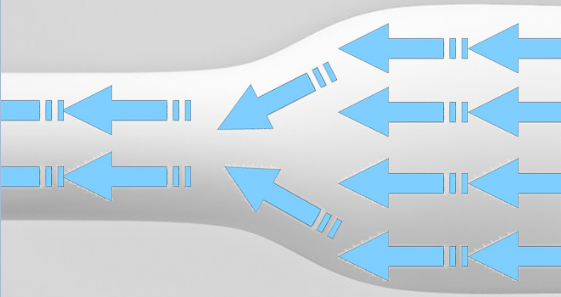
\includegraphics[scale=0.4]{CUELLOBOTELLA}
 					\caption{ Representación gráfica de un cuello de botella, tomada de [Aakvaag, 2006]}
				\end{figure}
				\end{center}
				\end{block}
	\end{frame}

	
% Diapositiva 4
\section{Adquisición de datos}
		\begin{frame}
			\frametitle{Process Simulator}			
	     	%Titulo Bloque.	
			\begin{block}{}
			    %Centrar
				\begin{center}
				ProModel Solutions  propone establecer un modelo de su sistema en una herramienta de simulación 3D.
				\begin{figure}[htb]
		    			
\includegraphics[scale=0.5]{pcs2014}
 					\caption{ Pantalla intro de Process Simulator 2014} 
				\end{figure}
				\end{center}
				
				%Para citar Biblografia, que se encuentra en el archivo .bib
				%\cite{Biblio1}
			\end{block}
			
	   	\end{frame}
		\begin{frame}
			\frametitle{Freeboard}			
	     	%Titulo Bloque.	
			\begin{block}{Estamos ante un panel web sencillo que muestra la información de los diferentes dispositivos que tengas conectados en tiempo real.}
			    %Centrar
				\begin{center}
				\begin{figure}[htb]
					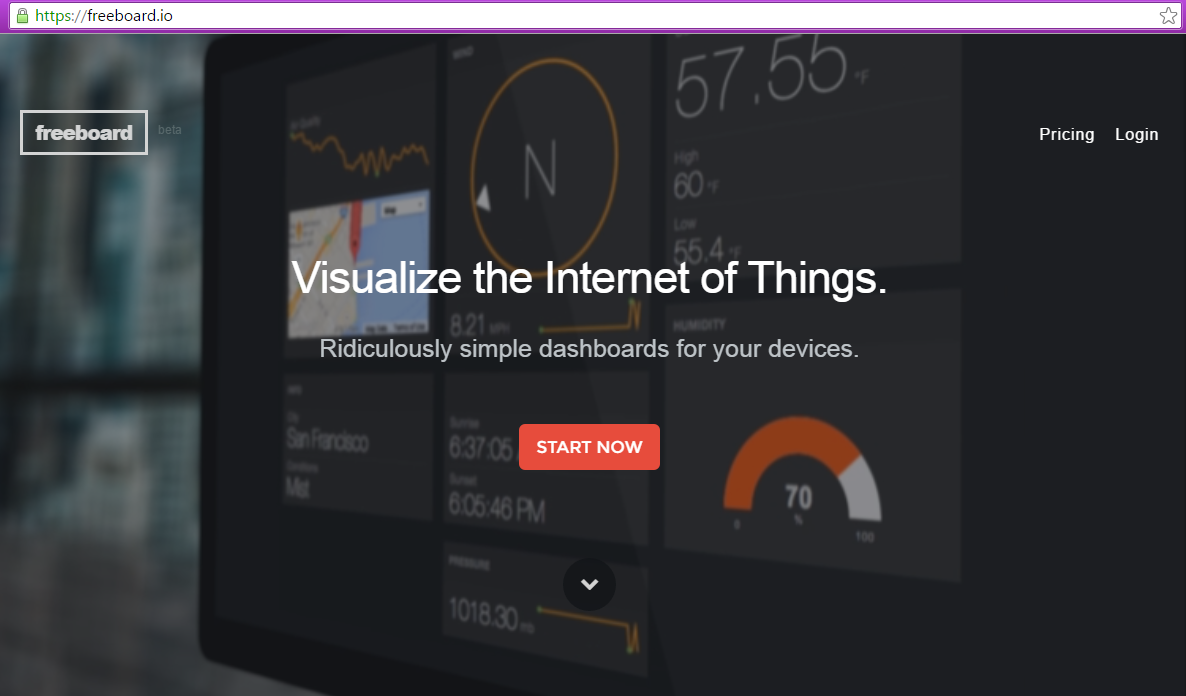
\includegraphics[scale=0.3]{freeboard} 
 					\caption{ Pantalla intro de freeboard.io}
				\end{figure}
				\end{center}
				
				%Para citar Biblografia, que se encuentra en el archivo .bib
				%\cite{Biblio1}
			\end{block}
			
	   	\end{frame}

		
% Diapositiva 6
		\begin{frame}
	    	\begin{block}{Simulación de cadena de suministro y proceso de producción}
			    %Centrar
				\begin{center}
				\begin{figure}[htb]
       			  		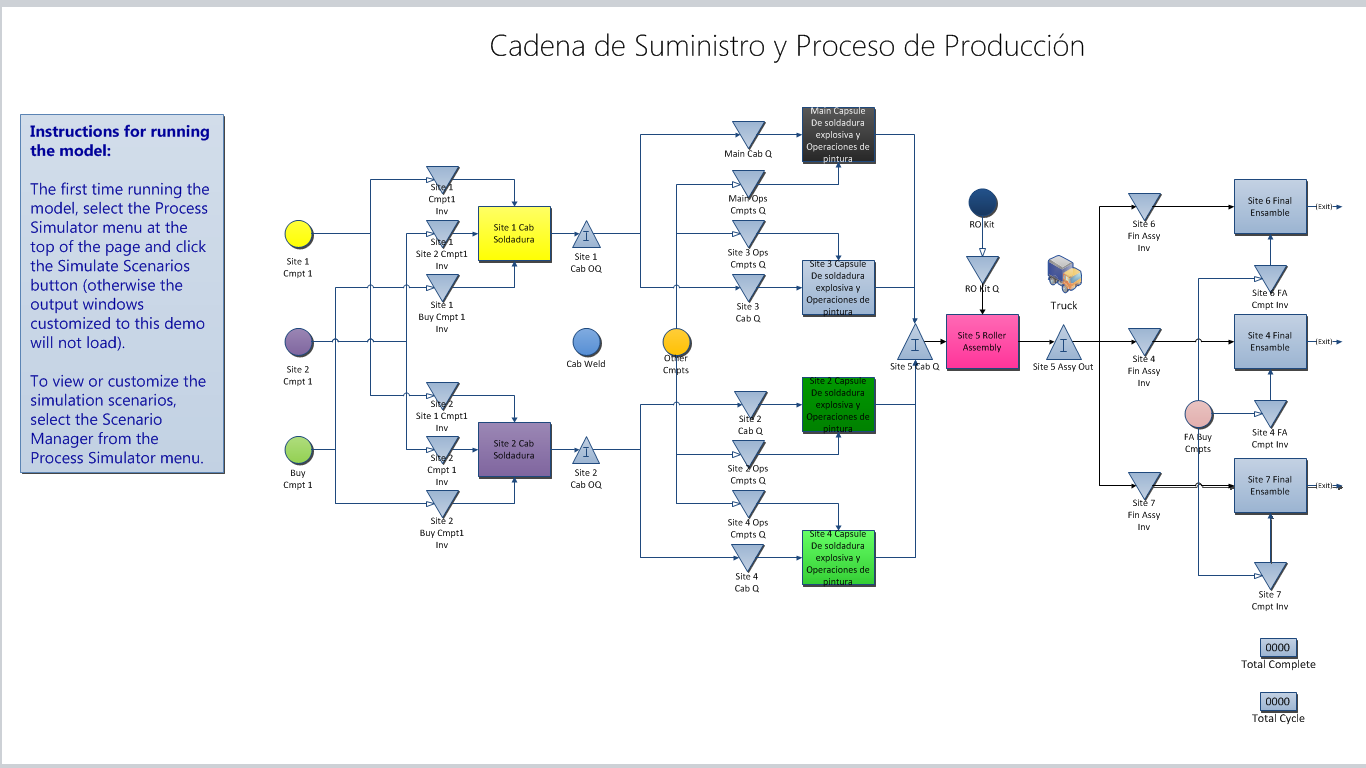
\includegraphics[scale=0.3]{procesodeproduccion}
					\caption{ \href{https://youtu.be/TfvSbhoqySw}{Esquema del proceso de producción a simular}} \label{fig:procesodeproduccion}
				\end{figure}
       				\end{center}
		   	\end{block}
		\end{frame}

% Diapositiva 7
\section{Resultados}	 
		\begin{frame}
    		\begin{block}{Resultados de Process Simulator}
				\begin{center}
				\begin{figure}[htb]
	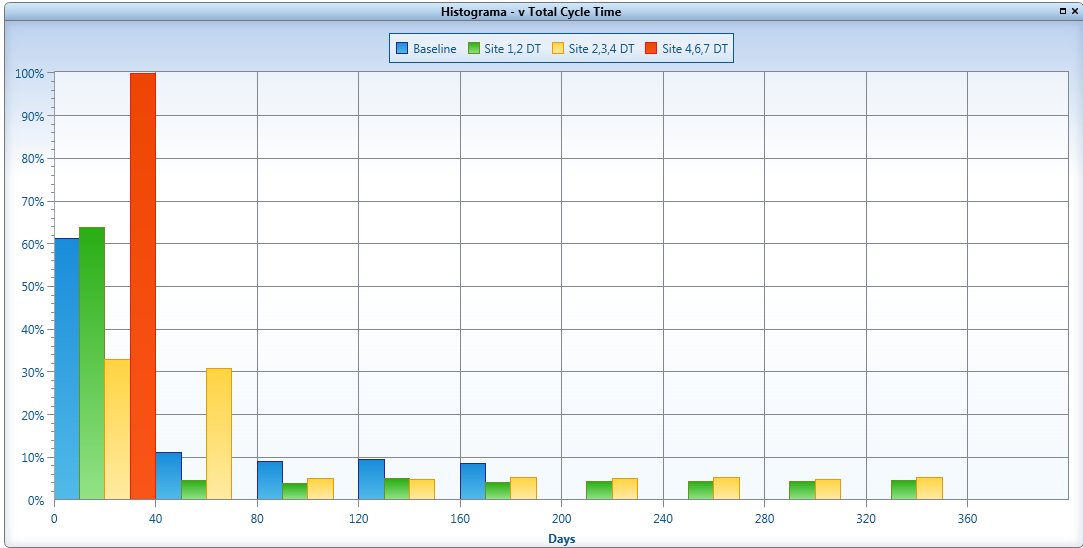
\includegraphics[width=\textwidth]{HISTOGRAMA}
	\caption{Histograma vs Ciclo Total de Tiempo}
	\label{fig:HISTOGRAMA}
				\end{figure}
				\end{center}
	   		\end{block}
	 	\end{frame}
		\begin{frame}
    		\begin{block}{Resultados de Freeboard}
				\begin{center}
				\begin{figure}[htb]
		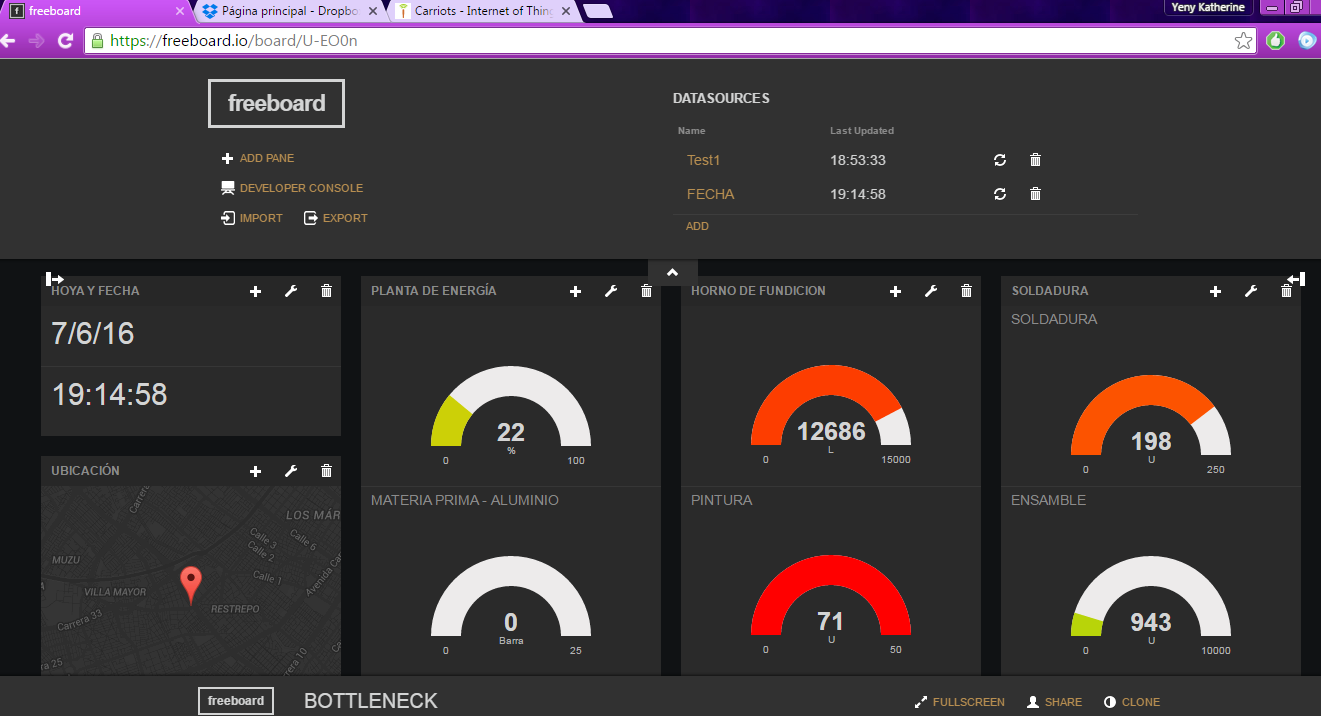
\includegraphics[scale=0.25]{RESULTADOS}   
	\caption{ \href{https://freeboard.io/board/U-EO0n}{Proceso de Producción en La Nube}} \label{fig:RESULTADOS}
				\end{figure}
				\end{center}
	   		\end{block}
	 	\end{frame}

% Diapositiva 7
\section{Conclusiones}	 
		\begin{frame}
    		\begin{block}{Conclusiones}
				\begin{center}
					Los cuellos de botella serán detectados a través de los análisis estadísticas de los resultados pero también visualizados a través de la animación. Esta última etapa permite darse cuenta del impacto de las acumulaciones sobre el sistema.
				\end{center}
	   		\end{block}
	 	\end{frame}
		
		
%BIBLIOGRAFIA
 \section{Bibliografía}
 	\begin{frame} 
 		\frametitle{Bibliografía}
	
\begin{thebibliography}{}

\bibitem[Yihui Xie, 2013]{Biblio1}
Yihui Xie (2013).
\newblock {\em Dynamic Documents with R and knitr}.
\newblock CRC Press 2016. 2 Ed.

\bibitem[Aakvaag, 2006]{Aakvaag2006}
Aakvaag, N. (2006).
\newblock {\em Redes de sensores inalambricos}.
\newblock Revista ABB

\bibitem[Ohri, 2014]{Ohri2014}
Ohri, A. (2014).
\newblock {\em R for Cloud Computing An Approach for Data Scientists}.
\newblock Springer Science+Business Media New York 2014

\end{thebibliography}

\end{frame}		
				
\end{document}